% Reduction graph of (\x.xx)(II) (generated by figs_c3ch05.py).
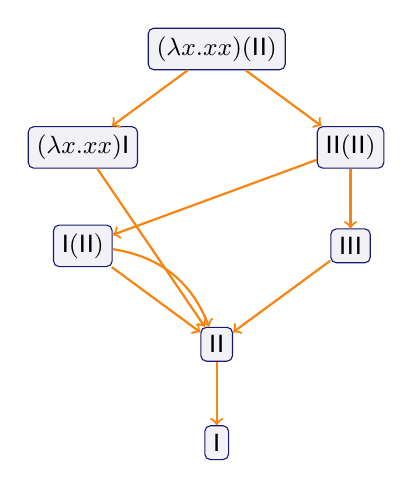
\begin{tikzpicture}[every node/.style={font=\small}]
\node[draw=MidnightBlue,rounded corners=2pt,fill=MidnightBlue!6,inner sep=3pt] (t0) at (0.00,-0.00) {$(\lambda x.xx)(\mathsf I\mathsf I)$};
\node[draw=MidnightBlue,rounded corners=2pt,fill=MidnightBlue!6,inner sep=3pt] (t2) at (-1.70,-1.25) {$(\lambda x.xx)\mathsf I$};
\node[draw=MidnightBlue,rounded corners=2pt,fill=MidnightBlue!6,inner sep=3pt] (t1) at (1.70,-1.25) {$\mathsf I\mathsf I(\mathsf I\mathsf I)$};
\node[draw=MidnightBlue,rounded corners=2pt,fill=MidnightBlue!6,inner sep=3pt] (t3) at (-1.70,-2.50) {$\mathsf I(\mathsf I\mathsf I)$};
\node[draw=MidnightBlue,rounded corners=2pt,fill=MidnightBlue!6,inner sep=3pt] (t4) at (1.70,-2.50) {$\mathsf I\mathsf I\mathsf I$};
\node[draw=MidnightBlue,rounded corners=2pt,fill=MidnightBlue!6,inner sep=3pt] (t5) at (0.00,-3.75) {$\mathsf I\mathsf I$};
\node[draw=MidnightBlue,rounded corners=2pt,fill=MidnightBlue!6,inner sep=3pt] (t6) at (0.00,-5.00) {$\mathsf I$};
\draw[->,thick,BurntOrange] (t0) -- (t1);
\draw[->,thick,BurntOrange] (t0) -- (t2);
\draw[->,thick,BurntOrange] (t1) -- (t3);
\draw[->,thick,BurntOrange] (t1) -- (t4);
\draw[->,thick,BurntOrange] (t2) -- (t5);
\draw[->,thick,BurntOrange] (t3) -- (t5);
\draw[->,thick,BurntOrange] (t3) to[bend left=30] (t5);
\draw[->,thick,BurntOrange] (t4) -- (t5);
\draw[->,thick,BurntOrange] (t5) -- (t6);
\end{tikzpicture}
